\documentclass[tikz,border=2pt]{standalone}
\usetikzlibrary{arrows.meta}

\begin{document}
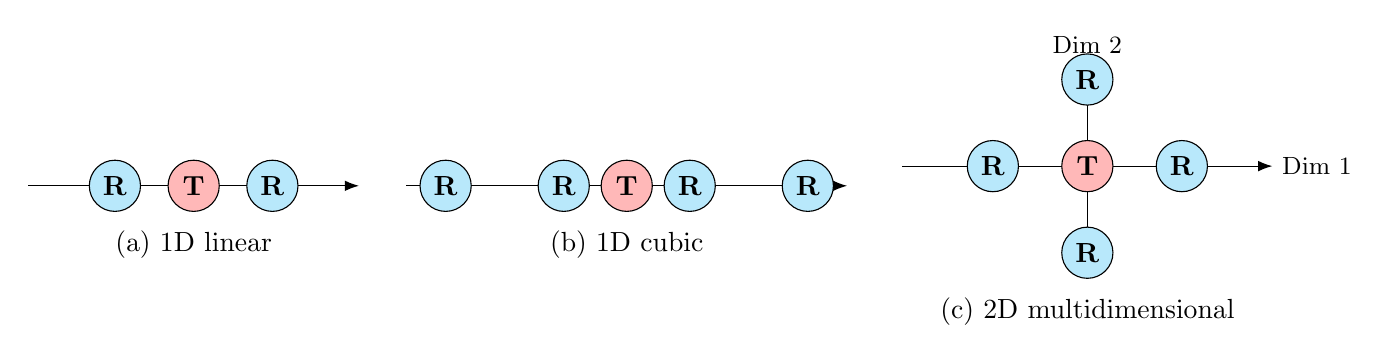
\begin{tikzpicture}[
reference/.style={circle,draw=black,fill=cyan!28,minimum size=6.5mm,inner sep=0pt,font=\bfseries},
target/.style={circle,draw=black,fill=red!28,minimum size=6.5mm,inner sep=0pt,font=\bfseries},
axis/.style={-{Latex[length=1.8mm]},line width=0.45pt}
]
\draw[axis](-0.1,1)--(4.1,1);
\node[reference]at(1,1){R};
\node[target]at(2,1){T};
\node[reference]at(3,1){R};
\node at(2,0.25){(a) 1D linear};

\draw[axis](4.7,1)--(10.3,1);
\node[reference]at(5.2,1){R};
\node[reference]at(6.7,1){R};
\node[target]at(7.5,1){T};
\node[reference]at(8.3,1){R};
\node[reference]at(9.8,1){R};
\node at(7.5,0.25){(b) 1D cubic};

\draw[axis](11,1.25)--(15.7,1.25)node[right]{\small Dim 1};
\draw[axis](13.35,-0.05)--(13.35,2.55)node[above]{\small Dim 2};
\node[target]at(13.35,1.25){T};
\node[reference]at(12.15,1.25){R};
\node[reference]at(14.55,1.25){R};
\node[reference]at(13.35,0.15){R};
\node[reference]at(13.35,2.35){R};
\node at(13.35,-0.6){(c) 2D multidimensional};
\end{tikzpicture}
\end{document}
